
\section{Создание экспериментального образца}

\subsection{Сборка квадрокоптера}
На основе компонентов, указанных в главе "Разработка архитектуры микродрона" собирается квадрокоптер. На раму устанавливаются все обозначенные компоненты. Фазы каждого мотора припаиваются на соответствующие площадки регуляторов. При проверке вращения моторов в случае несоответствия вращения мотора схеме для px4, необходимо перепаять любые две фазы этого мотора. Также к регуляторам припаиваются силовые провода с коннектором для подключения аккумулятора. Полетный контроллер располагается на виброизоляционных прокладках и подключается к регуляторам через колодку. Далее производится монтаж FPV оборудования, приемника и телеметрийного модуля (рис. \ref{fig:quad1}).
% ~\ref{fig:quad1}
\begin{figure}[H]
	\centering
	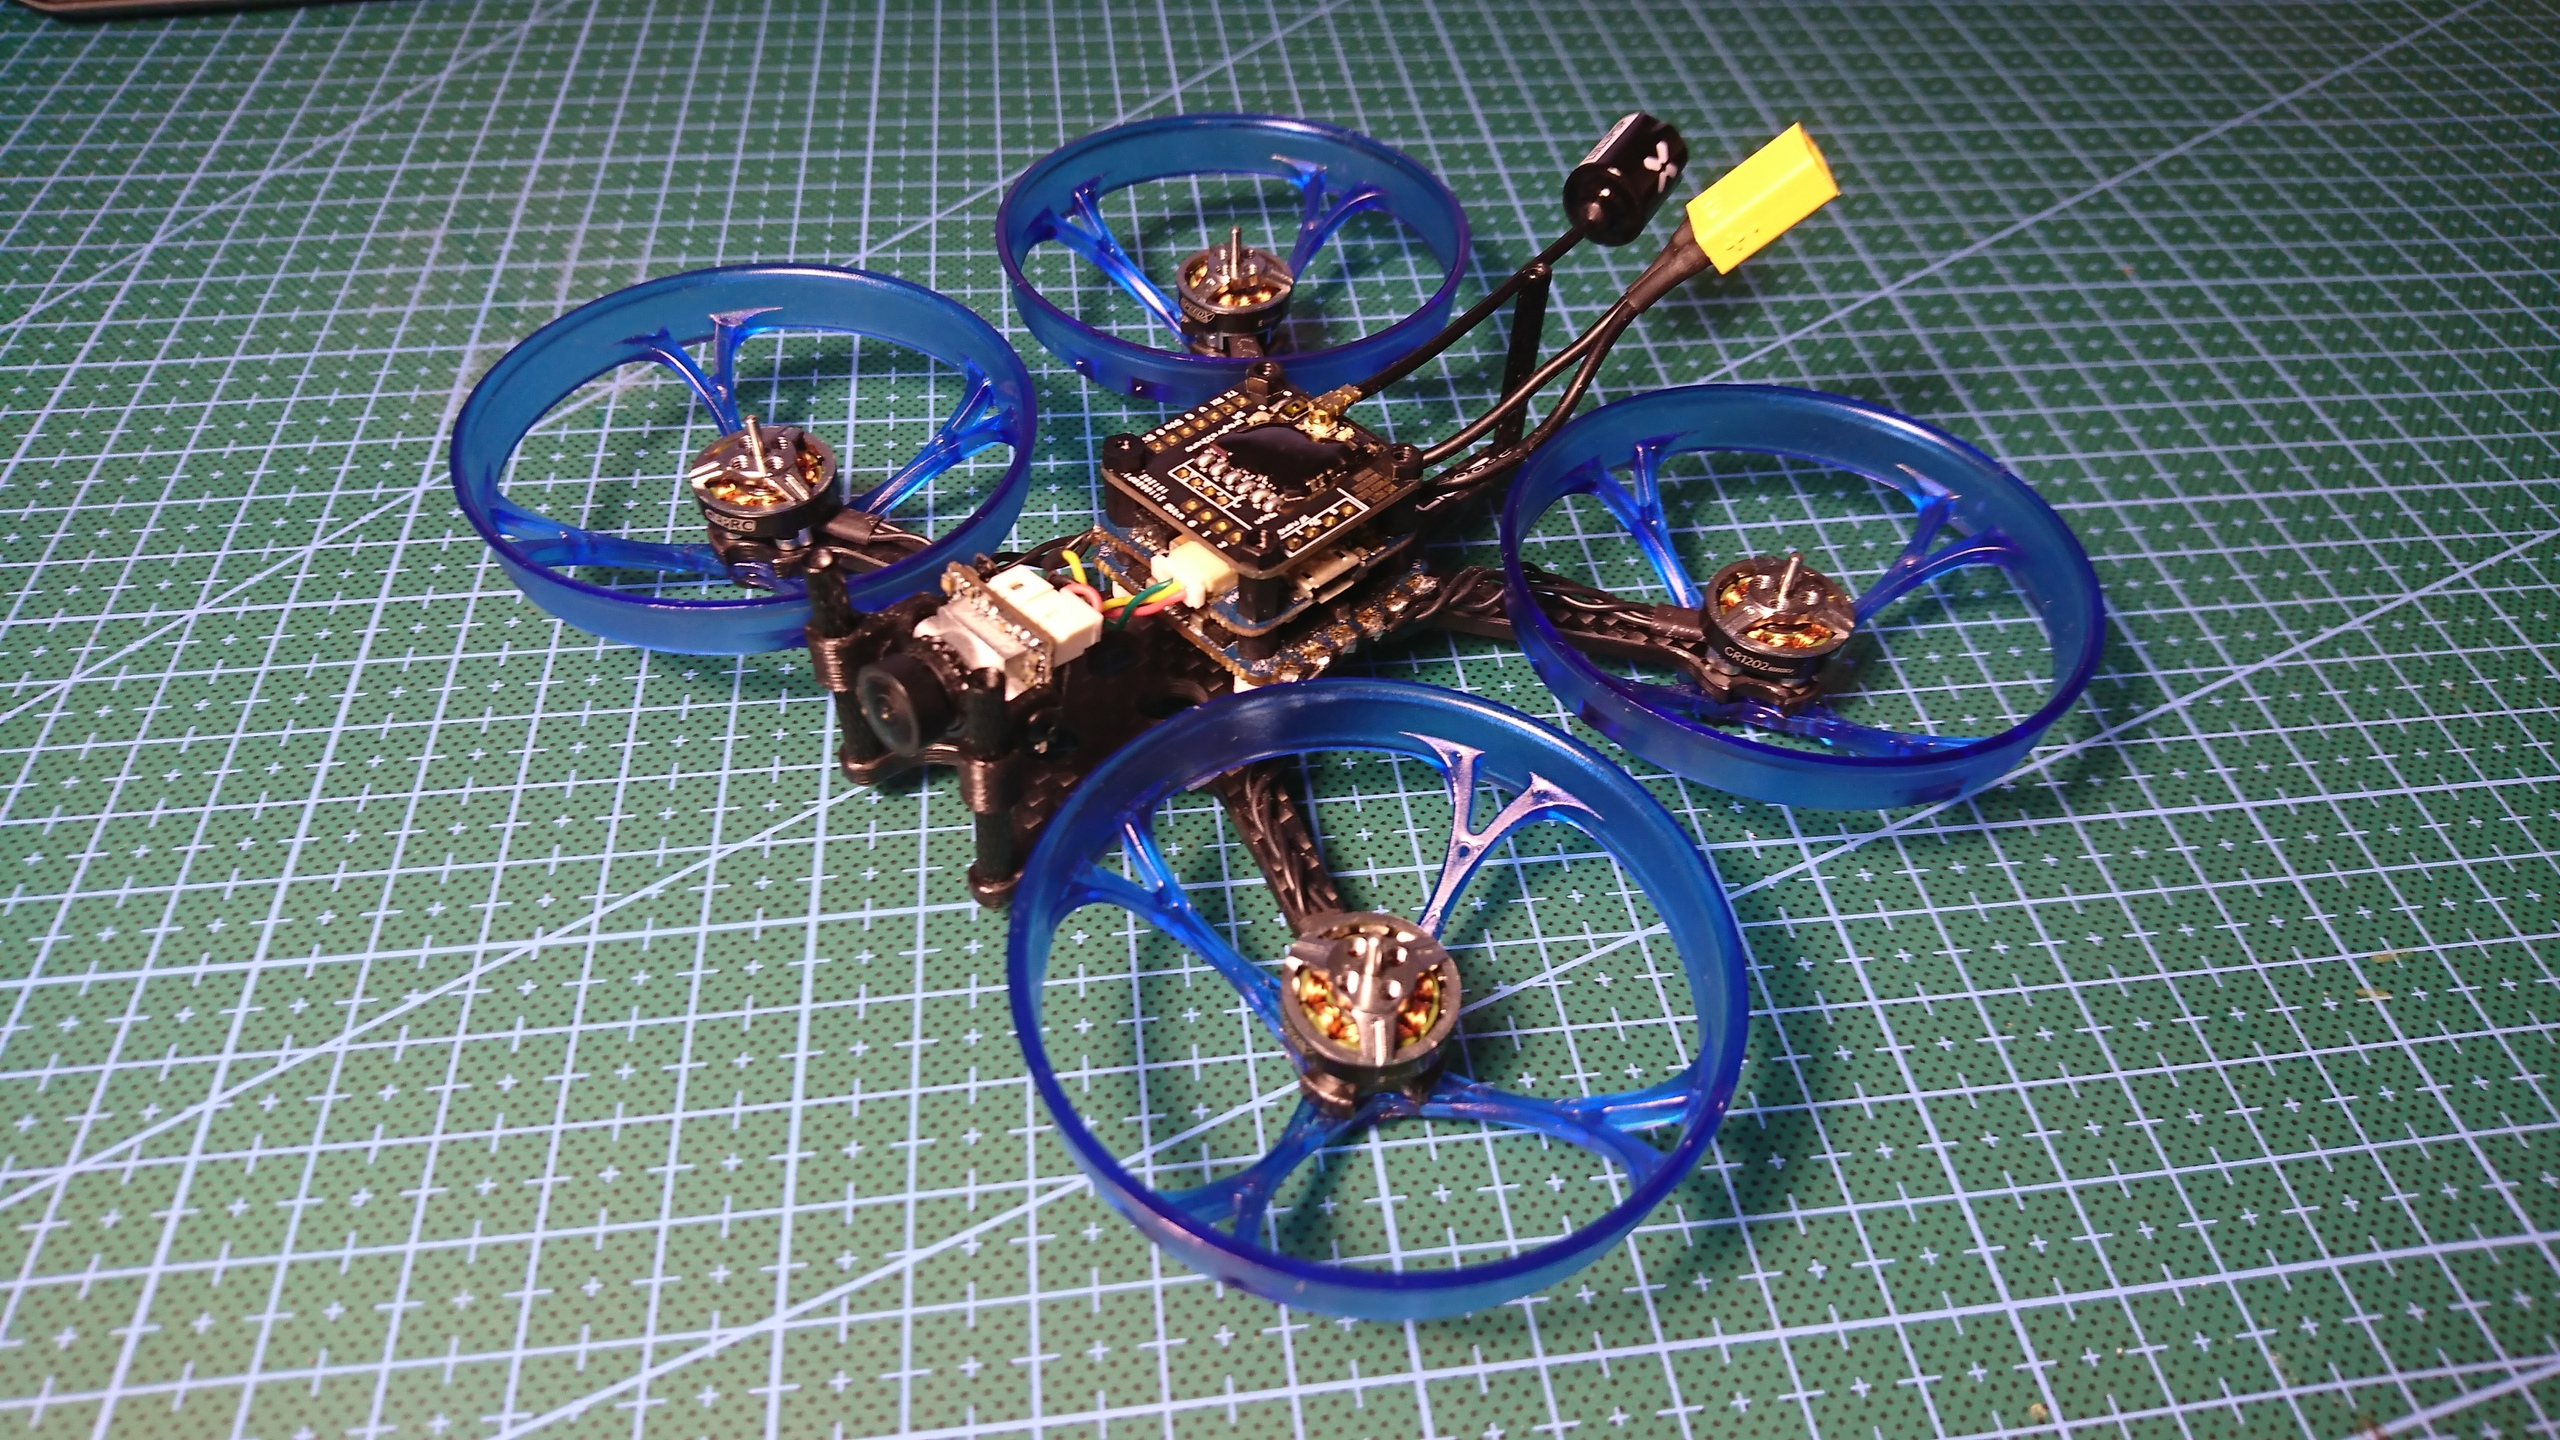
\includegraphics[width=0.5\linewidth]{pics/quad1}
	\caption{Установка компонентов на раму
	}
	\label{fig:quad1}
\end{figure}
Прикручивается верхняя пластина рамы, закрепляются все свисающие детали и на этом сборка завершается (рис. \ref{fig:quad2}).
% ~\ref{fig:quad2}
\begin{figure}[H]
	\centering
	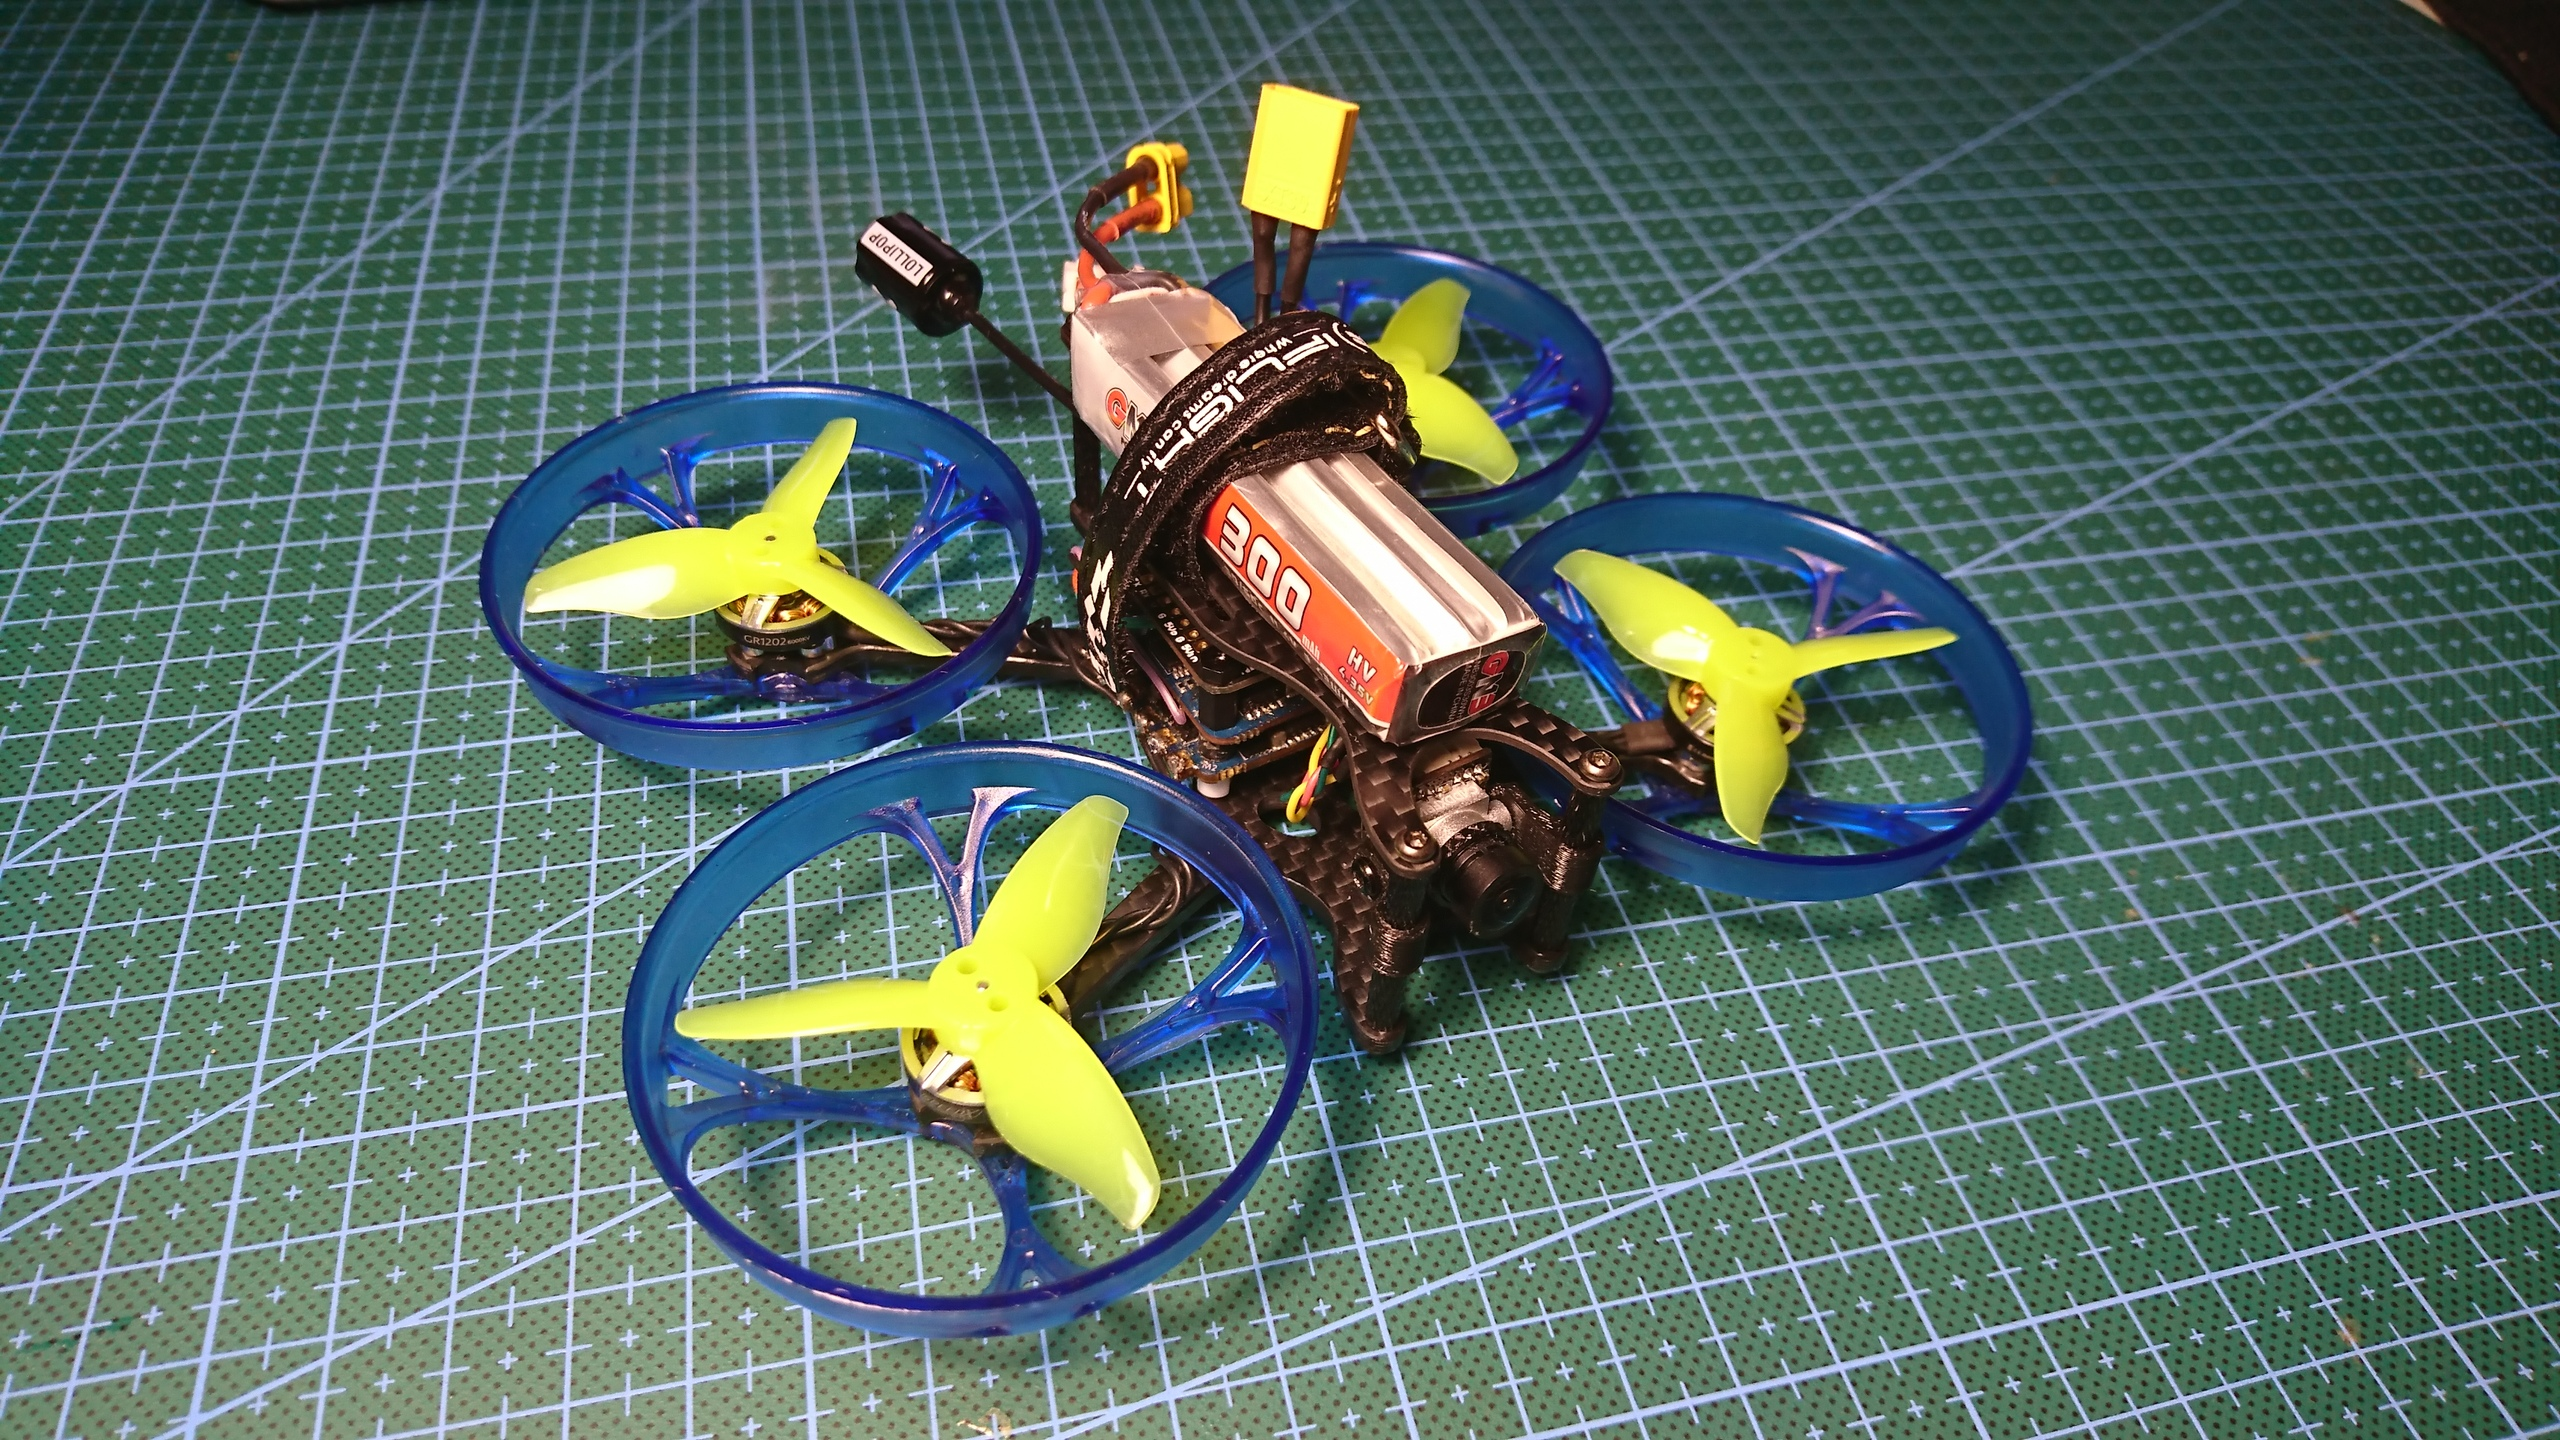
\includegraphics[width=0.5\linewidth]{pics/quad2}
	\caption{Экспериментальный образец квадрокоптера
	}
	\label{fig:quad2}
\end{figure}

\subsection{Сборка наземной станции}
Согласно шагам из главы "Разработка архитектуры наземной станции" про\-из\-водится подключение всех компонентов наземной станции.
\subsection{Обновление и настройка параметров ПО}
На полетный контроллер через qgroundcontrol по USB прошивается последний образ PX4 из репозитория clover. Производится калибровка всех датчиков. Для взаимодействия приемника с радиомодулем требуется выполнение процедуры привязки -- bind.
Настраиваются бод -- рейты устройств приема-передачи телеметрии на максимально доступное значение. Для экспериментального образца использовались устройства 3DR с бод -- рейтами 115200. При подключении через 3DR модули параметры квадрокоптера считались и отобразились в конфигураторе. Остается настройка базовой станции. Видеоприемник настраивается на диапазон частот видеопередатчика в режиме автопоиска сигнала. Окружение для наземной станции создавалось на базе пакета clover, где предустановлены все необходимые инструменты. В launch файлах меняются параметры для способа подключения, чтобы была доступна симуляция окружения квадрокоптера. Для топика указывается порт, к которому подключен видеомодуль. После перезагрузки применяются параметры и можно приступать к тестированию.
\subsection{Проверка работы экспериментального образца}
Для проверки работы aruco\_detect создается карта маркеров, прописанная в конфигурационном файле пакета clover (рис. \ref{fig:map}).
% ~\ref{fig:map}
\begin{figure}[H]
	\centering
	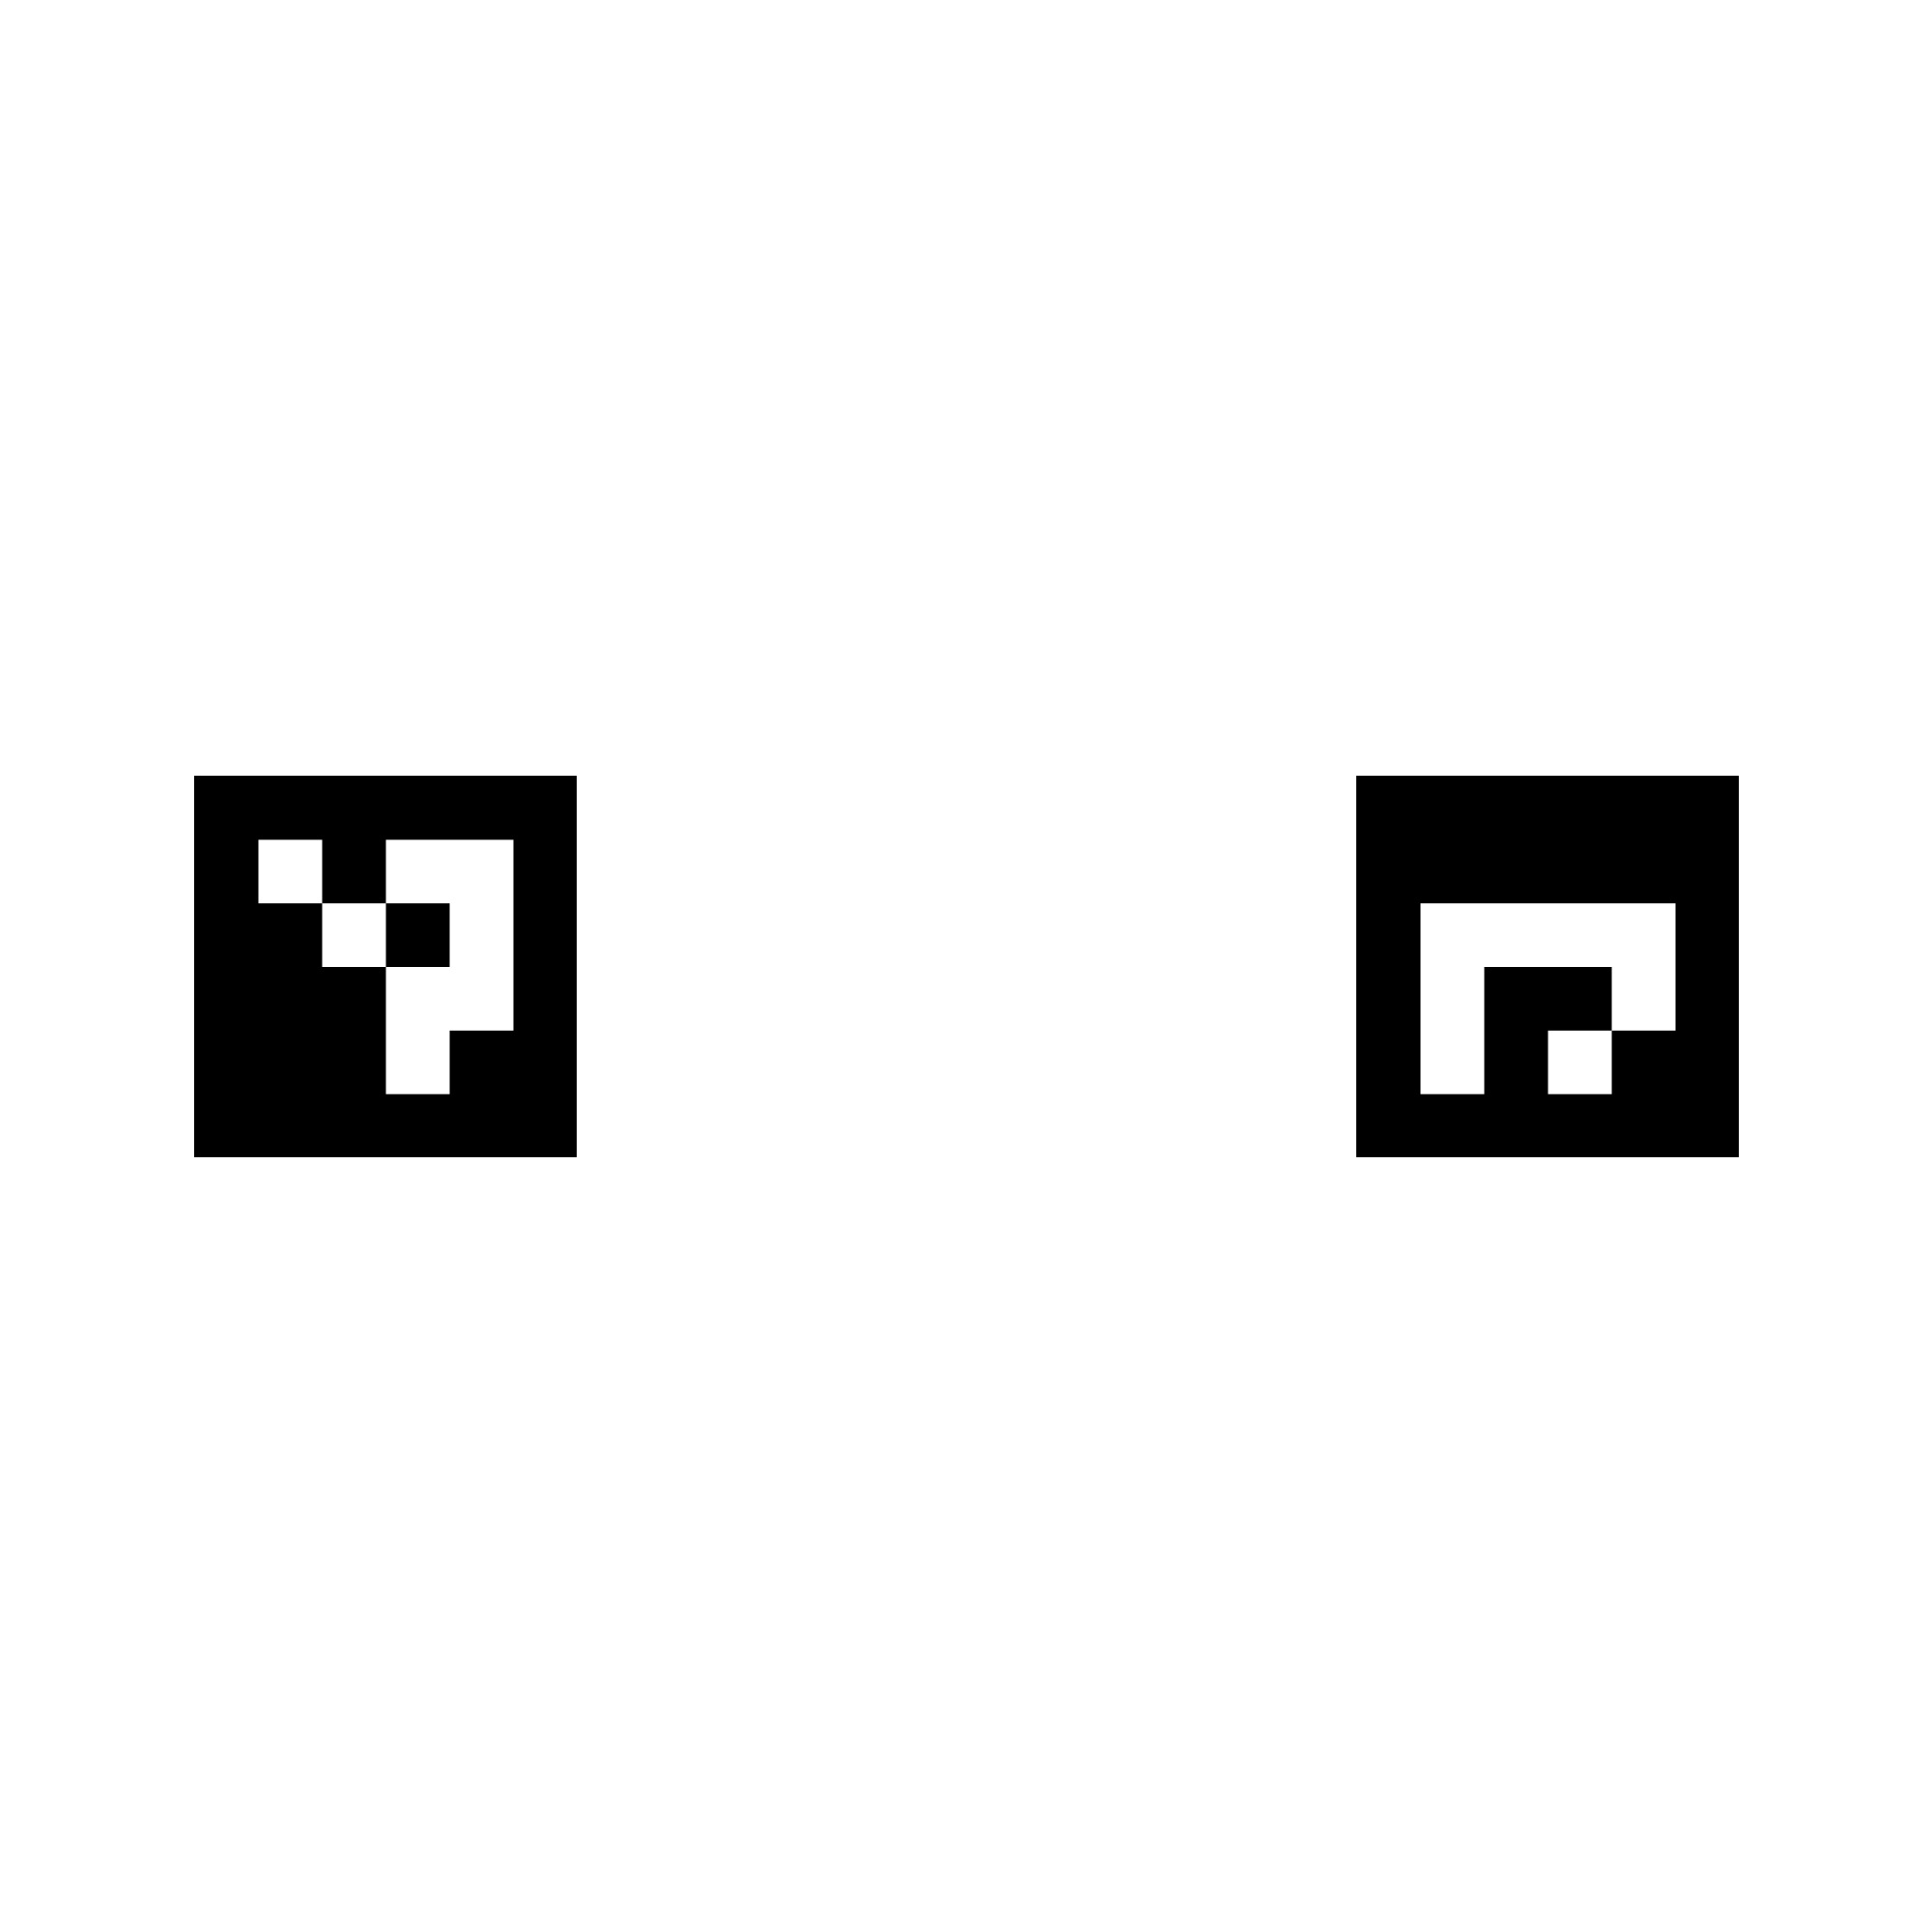
\includegraphics[width=0.5\linewidth]{pics/map}
	\caption{Карта маркеров
	}
	\label{fig:map}
\end{figure}
Наводим камеру квадрокоптера на метки, проверяем топик aruco\_detect и получаем идентификаторы меток (рис. \ref{fig:aruco_detect}).
% ~\ref{fig:aruco_detect}
\begin{figure}[H]
	\centering
	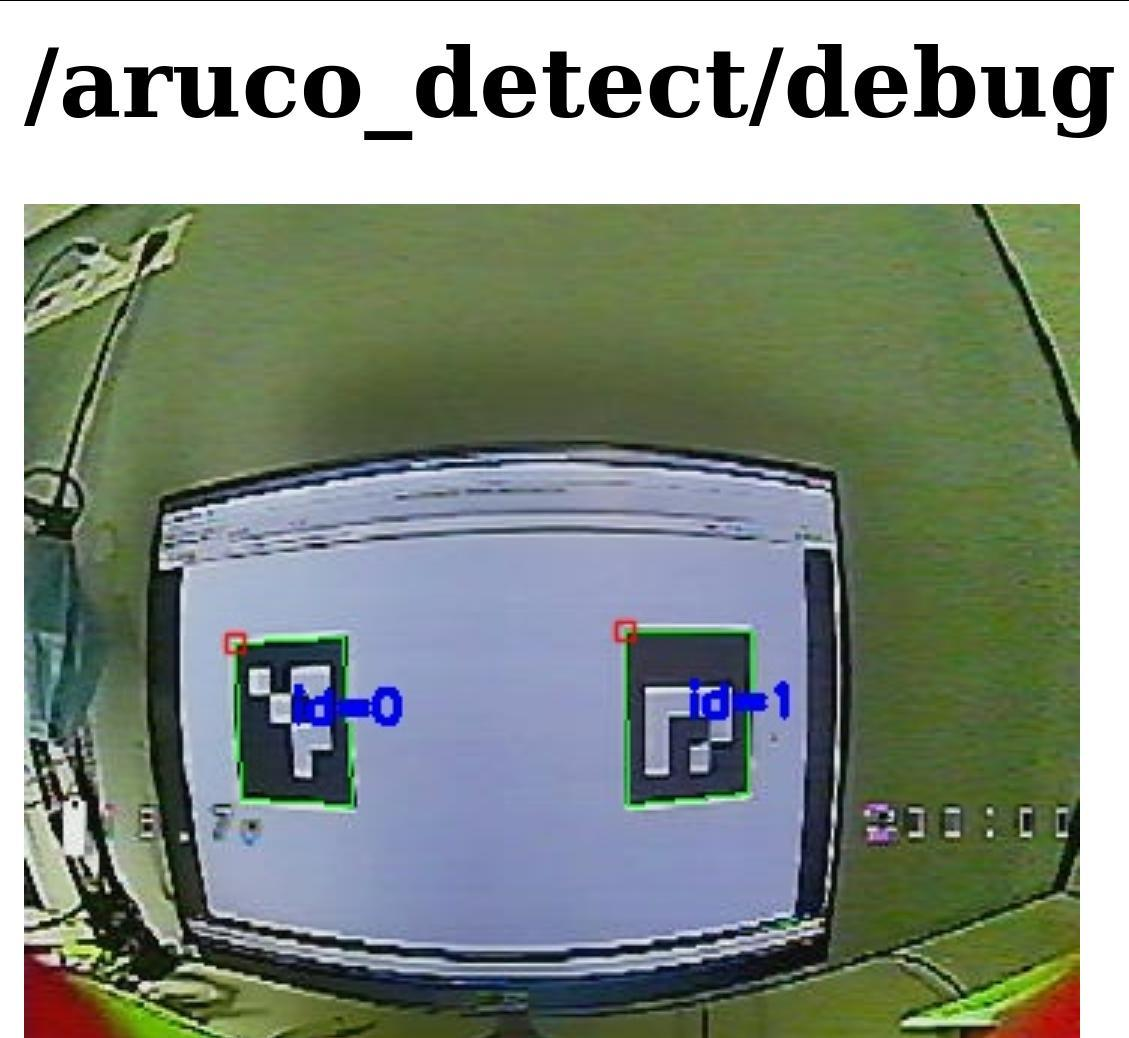
\includegraphics[width=0.5\linewidth]{pics/aruco_detect}
	\caption{Инициализация aruco маркеров
	}
	\label{fig:aruco_detect}
\end{figure}
Замеряем задержку (рис. \ref{fig:time}).
% ~\ref{fig:time}
\begin{figure}[H]
	\centering
	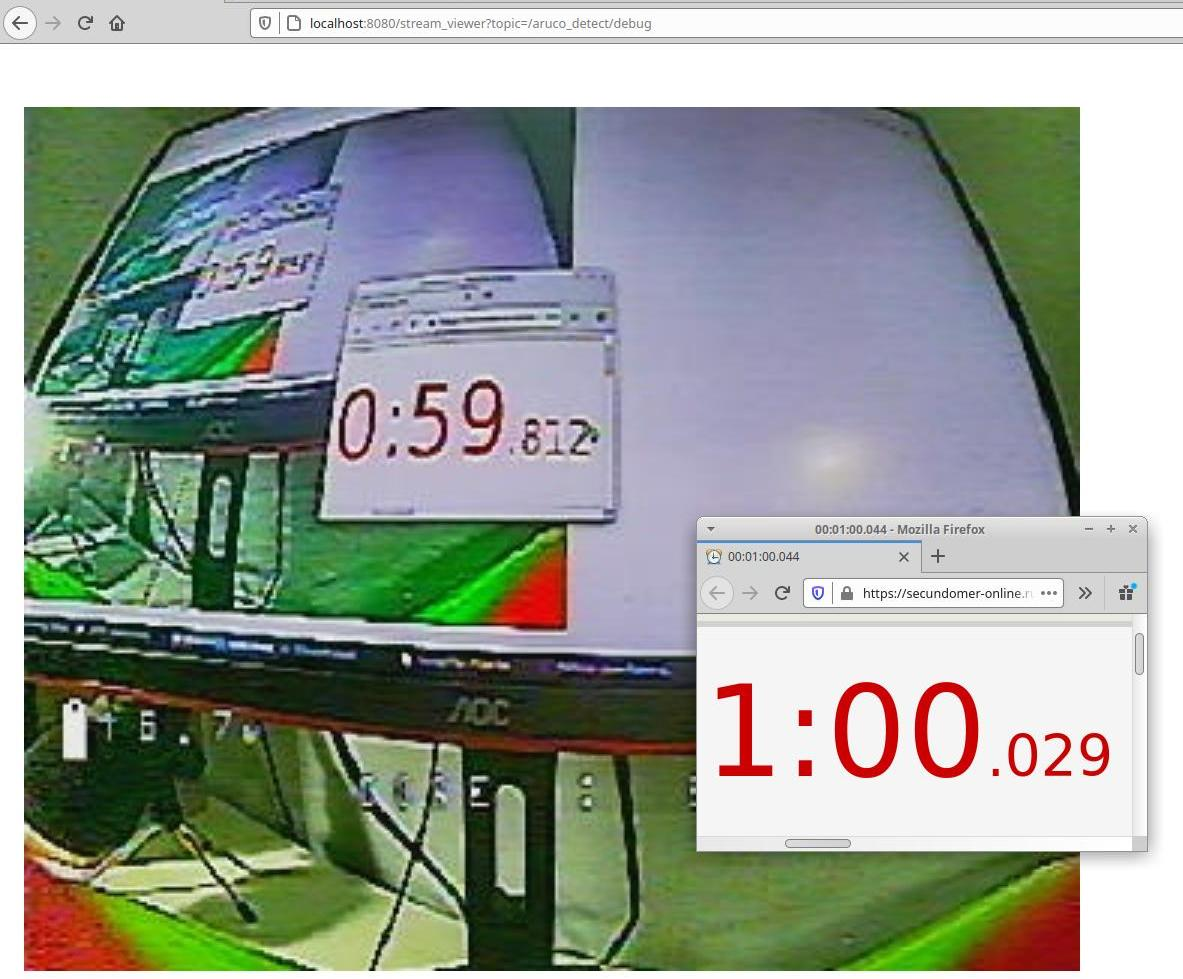
\includegraphics[width=0.5\linewidth]{pics/time}
	\caption{Время задержки% 0.2с
	}
	\label{fig:time}
\end{figure}
В теории, уже сейчас квадрокоптер готов к выполнению автономного полета. Однако из тестов видно, что задержка составляет порядка 200 мс, что критично для позиционирования квадрокоптера. Такая задержка обусловлена суммой задержек каждого устройства (камеры, видеопередатчика, видеоприемника, USB порта компьютера). Учитывая, что задержка также присутствует на устройстве приема-передачи телеметрии, обнаруживается критичная проблема у разрабатываемого комплекта. Уменьшение задержки -- одна из сложнейших задач, решению которых будет посвящен следующий этап исследования. Предполагаемые пути, которые позволят снизить задержки следующие:

--- подключение модуля телеметрии с более высоким бод -- рейтом;

--- модификация MAVLink протокола под наши нужды;

--- использование модификации MAVLink в виде fast-RTPS, включая уровень для преобразования сообщений uORB PX4.

Также огромной проблемой является качество и задержка видеоканала. Решение этой проблемы может быть в использовании цифровой системы передачи видеопотока, например, OpenHD \cite{openhd}.

